\def\EmbedPictsWidth{2.5}
\def\EmbedPictsMargin{1}
\def\EmbedPictsTxtSize{}
\begin{frame}
\frametitle{Embedded events}
\begin{center}
\begin{tikzpicture}
\draw (\EmbedPictsWidth/2, \EmbedPictsWidth) node [above] {\EmbedPictsTxtSize $\Zboson\to\mu\mu$ data};
\node[anchor=south west,inner sep=0] at (0,0) {\frame{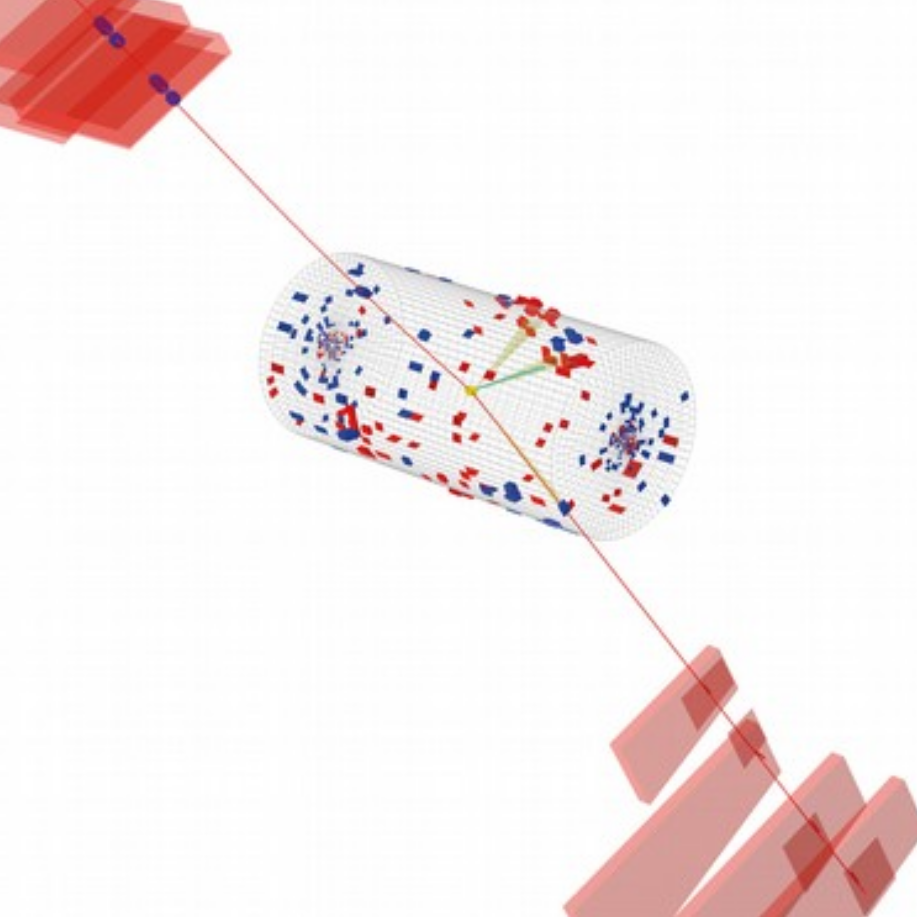
\includegraphics[width=\EmbedPictsWidth cm]{\PhDthesisdir/tex/slides/HTT_analysis/embedding_explained/Z_to_mumu_data.png}}};

%\draw [-latex, very thick] (\EmbedPictsWidth+\EmbedPictsMargin/5, \EmbedPictsWidth/2) -- + (3*\EmbedPictsMargin/5,0);
%\draw (\EmbedPictsWidth/2+\EmbedPictsWidth+\EmbedPictsMargin, \EmbedPictsWidth) node [above] {\EmbedPictsTxtSize Remove $\mu\mu$ system};
%\node[anchor=south west,inner sep=0] at (\EmbedPictsWidth+\EmbedPictsMargin,0) {\frame{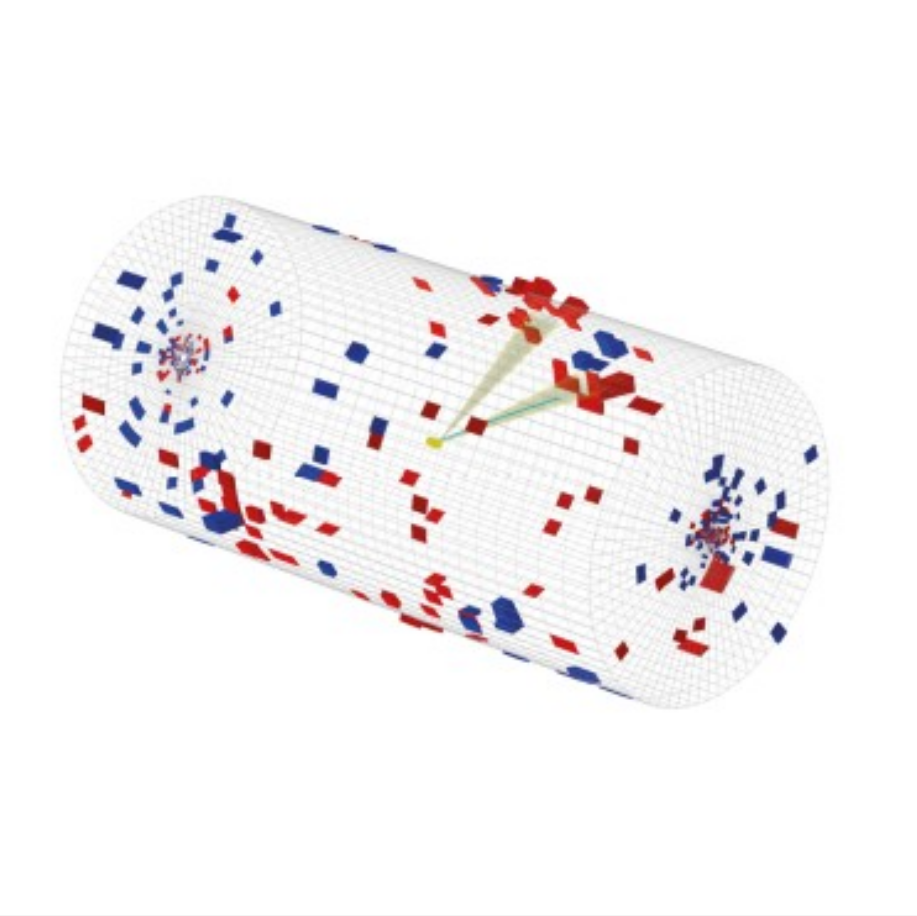
\includegraphics[width=\EmbedPictsWidth cm]{\PhDthesisdir/tex/slides/HTT_analysis/embedding_explained/remove_mumu.png}}};
%
%\draw (\EmbedPictsWidth+\EmbedPictsMargin,-\EmbedPictsWidth/2-\EmbedPictsMargin) node [above left] {\EmbedPictsTxtSize Simulate $\Zboson\to\tau\tau$};
%\draw (\EmbedPictsWidth+\EmbedPictsMargin,-\EmbedPictsWidth/2-\EmbedPictsMargin) node [below left] {\EmbedPictsTxtSize (\tau\ with same kinematics as \mu)};
%\node[anchor=south west,inner sep=0] at (\EmbedPictsWidth+\EmbedPictsMargin,-\EmbedPictsWidth-\EmbedPictsMargin) {\frame{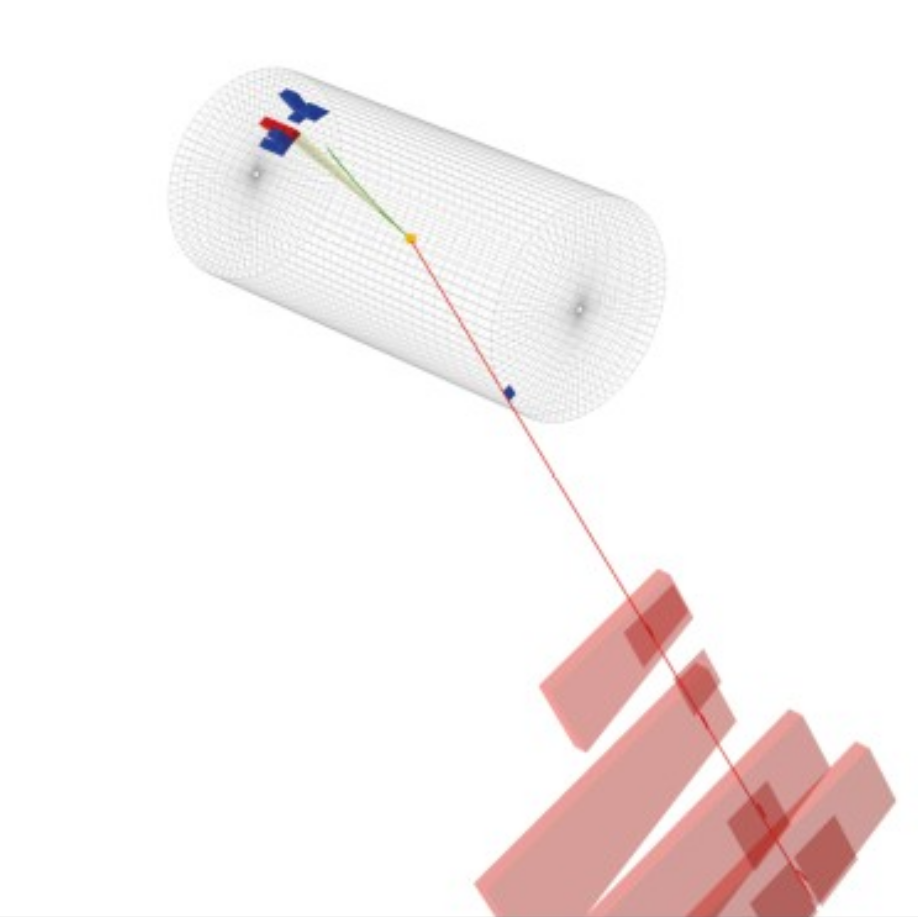
\includegraphics[width=\EmbedPictsWidth cm]{\PhDthesisdir/tex/slides/HTT_analysis/embedding_explained/Z_to_tautau_simulation.png}}};
%
%\draw [-latex, very thick] (2*\EmbedPictsWidth+6*\EmbedPictsMargin/5, \EmbedPictsWidth/4) -- (2*\EmbedPictsWidth+2*\EmbedPictsMargin-\EmbedPictsMargin/5,0);
%\draw [-latex, very thick] (2*\EmbedPictsWidth+6*\EmbedPictsMargin/5,-\EmbedPictsWidth/4-\EmbedPictsMargin) -- (2*\EmbedPictsWidth+2*\EmbedPictsMargin-\EmbedPictsMargin/5,-\EmbedPictsMargin);
%\draw (2*\EmbedPictsWidth+2*\EmbedPictsMargin+\EmbedPictsWidth/2,\EmbedPictsWidth/2-\EmbedPictsMargin/2) node [above] {\EmbedPictsTxtSize $\Zboson\to\tau\tau$ embedded event};
%\node[anchor=south west,inner sep=0] at (2*\EmbedPictsWidth+2*\EmbedPictsMargin,-\EmbedPictsWidth/2-\EmbedPictsMargin/2) {\frame{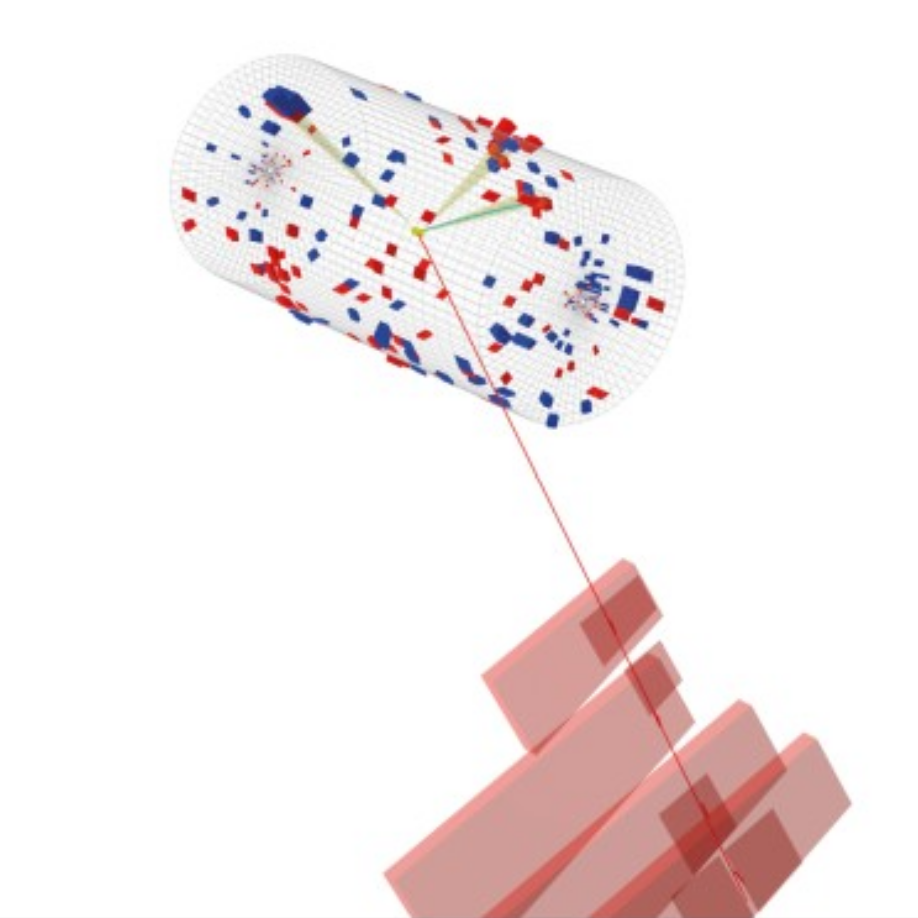
\includegraphics[width=\EmbedPictsWidth cm]{\PhDthesisdir/tex/slides/HTT_analysis/embedding_explained/embedded_event.png}}};

\clip (-1,-\EmbedPictsWidth-\EmbedPictsMargin-.25) rectangle (3*\EmbedPictsWidth+5*\EmbedPictsMargin/2+.25, \EmbedPictsWidth+.5);
\end{tikzpicture}
\end{center}
\end{frame}

\begin{frame}\addtocounter{framenumber}{-1}
\frametitle{Embedded events}
\begin{center}
\begin{tikzpicture}
\draw (\EmbedPictsWidth/2, \EmbedPictsWidth) node [above] {\EmbedPictsTxtSize $\Zboson\to\mu\mu$ data};
\node[anchor=south west,inner sep=0] at (0,0) {\frame{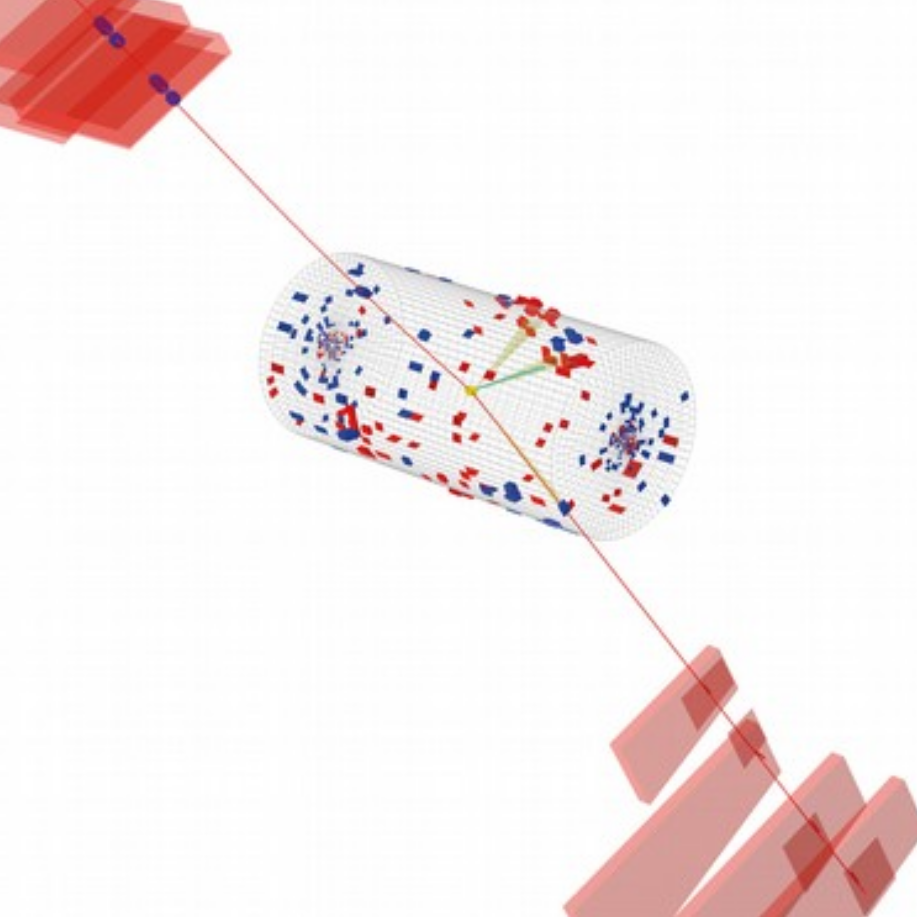
\includegraphics[width=\EmbedPictsWidth cm]{\PhDthesisdir/tex/slides/HTT_analysis/embedding_explained/Z_to_mumu_data.png}}};

\draw [-latex, very thick] (\EmbedPictsWidth+\EmbedPictsMargin/5, \EmbedPictsWidth/2) -- + (3*\EmbedPictsMargin/5,0);
\draw (\EmbedPictsWidth/2+\EmbedPictsWidth+\EmbedPictsMargin, \EmbedPictsWidth) node [above] {\EmbedPictsTxtSize Remove $\mu\mu$ system};
\node[anchor=south west,inner sep=0] at (\EmbedPictsWidth+\EmbedPictsMargin,0) {\frame{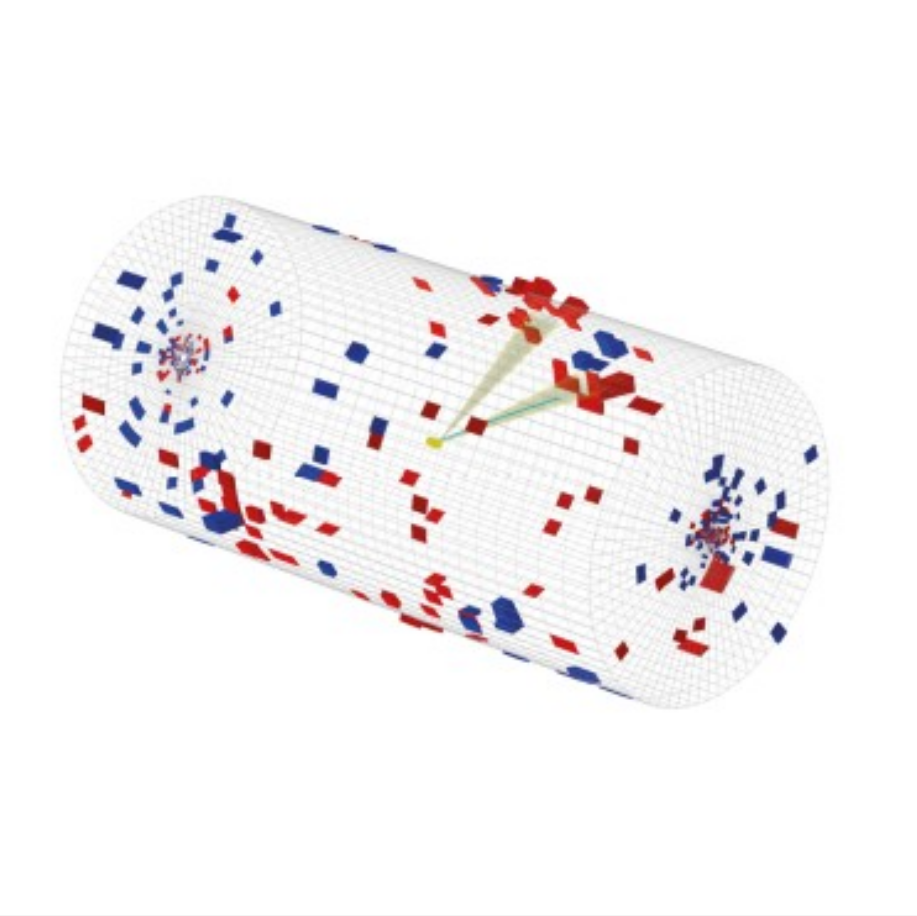
\includegraphics[width=\EmbedPictsWidth cm]{\PhDthesisdir/tex/slides/HTT_analysis/embedding_explained/remove_mumu.png}}};

%\draw (\EmbedPictsWidth+\EmbedPictsMargin,-\EmbedPictsWidth/2-\EmbedPictsMargin) node [above left] {\EmbedPictsTxtSize Simulate $\Zboson\to\tau\tau$};
%\draw (\EmbedPictsWidth+\EmbedPictsMargin,-\EmbedPictsWidth/2-\EmbedPictsMargin) node [below left] {\EmbedPictsTxtSize (\tau\ with same kinematics as \mu)};
%\node[anchor=south west,inner sep=0] at (\EmbedPictsWidth+\EmbedPictsMargin,-\EmbedPictsWidth-\EmbedPictsMargin) {\frame{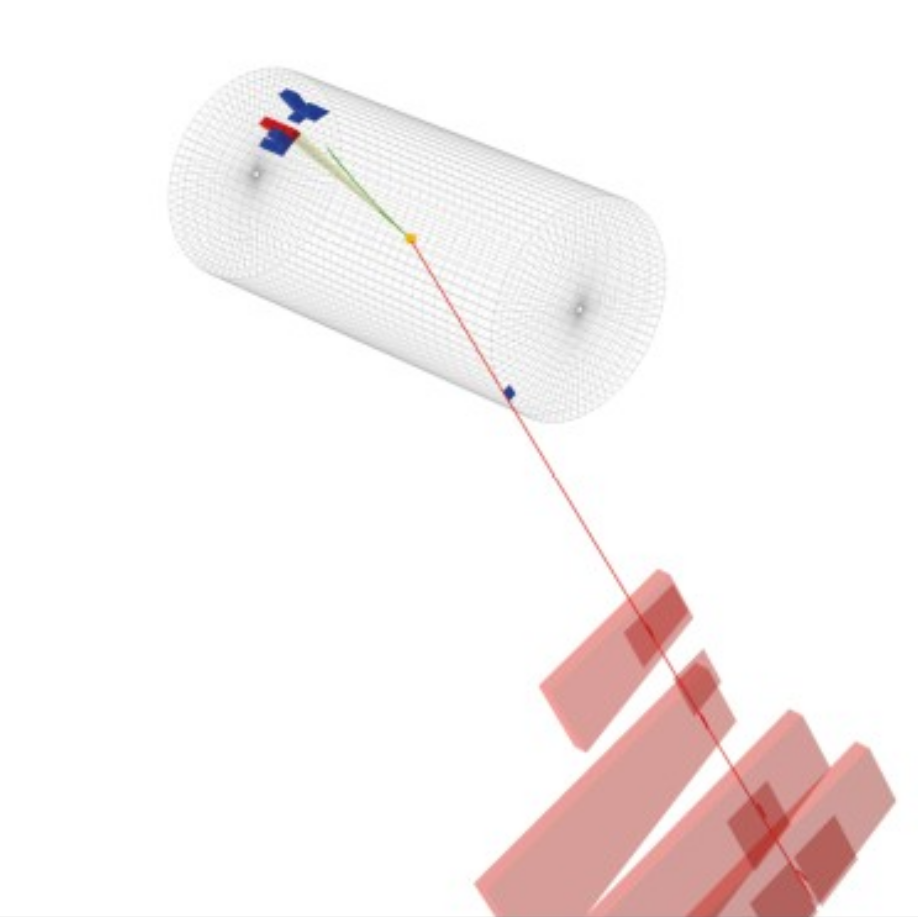
\includegraphics[width=\EmbedPictsWidth cm]{\PhDthesisdir/tex/slides/HTT_analysis/embedding_explained/Z_to_tautau_simulation.png}}};
%
%\draw [-latex, very thick] (2*\EmbedPictsWidth+6*\EmbedPictsMargin/5, \EmbedPictsWidth/4) -- (2*\EmbedPictsWidth+2*\EmbedPictsMargin-\EmbedPictsMargin/5,0);
%\draw [-latex, very thick] (2*\EmbedPictsWidth+6*\EmbedPictsMargin/5,-\EmbedPictsWidth/4-\EmbedPictsMargin) -- (2*\EmbedPictsWidth+2*\EmbedPictsMargin-\EmbedPictsMargin/5,-\EmbedPictsMargin);
%\draw (2*\EmbedPictsWidth+2*\EmbedPictsMargin+\EmbedPictsWidth/2,\EmbedPictsWidth/2-\EmbedPictsMargin/2) node [above] {\EmbedPictsTxtSize $\Zboson\to\tau\tau$ embedded event};
%\node[anchor=south west,inner sep=0] at (2*\EmbedPictsWidth+2*\EmbedPictsMargin,-\EmbedPictsWidth/2-\EmbedPictsMargin/2) {\frame{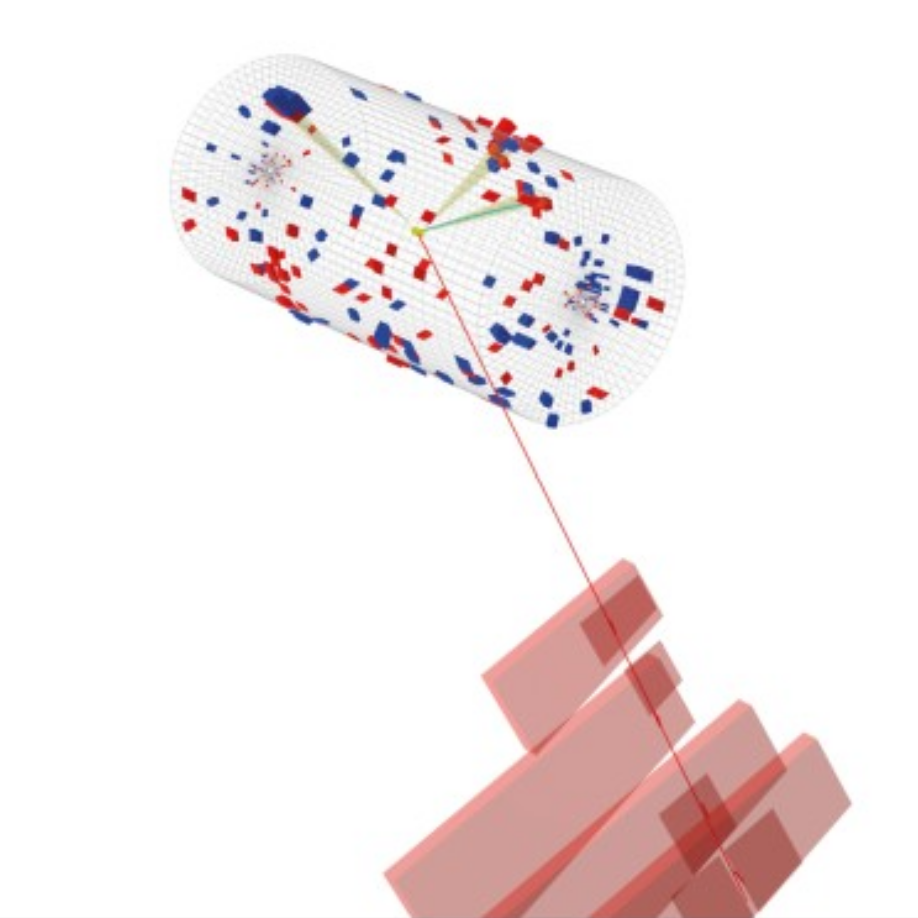
\includegraphics[width=\EmbedPictsWidth cm]{\PhDthesisdir/tex/slides/HTT_analysis/embedding_explained/embedded_event.png}}};

\clip (-1,-\EmbedPictsWidth-\EmbedPictsMargin-.25) rectangle (3*\EmbedPictsWidth+5*\EmbedPictsMargin/2+.25, \EmbedPictsWidth+.5);
\end{tikzpicture}
\end{center}
\end{frame}

\begin{frame}\addtocounter{framenumber}{-1}
\frametitle{Embedded events}
\begin{center}
\begin{tikzpicture}
\draw (\EmbedPictsWidth/2, \EmbedPictsWidth) node [above] {\EmbedPictsTxtSize $\Zboson\to\mu\mu$ data};
\node[anchor=south west,inner sep=0] at (0,0) {\frame{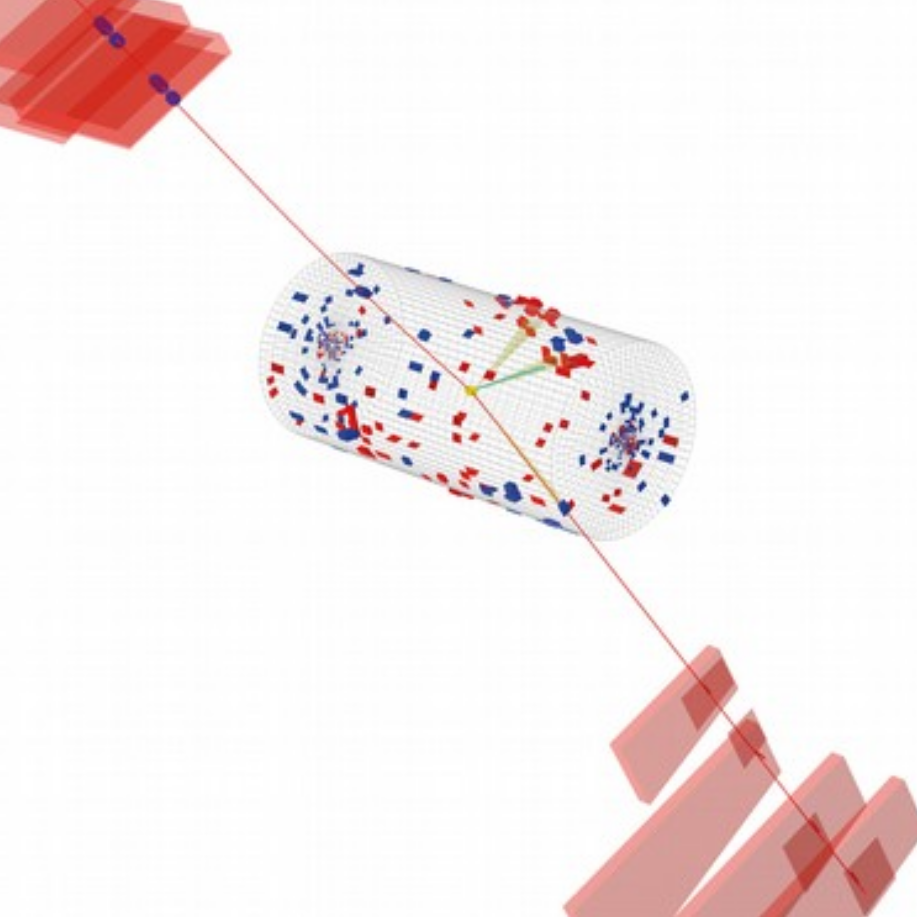
\includegraphics[width=\EmbedPictsWidth cm]{\PhDthesisdir/tex/slides/HTT_analysis/embedding_explained/Z_to_mumu_data.png}}};

\draw [-latex, very thick] (\EmbedPictsWidth+\EmbedPictsMargin/5, \EmbedPictsWidth/2) -- + (3*\EmbedPictsMargin/5,0);
\draw (\EmbedPictsWidth/2+\EmbedPictsWidth+\EmbedPictsMargin, \EmbedPictsWidth) node [above] {\EmbedPictsTxtSize Remove $\mu\mu$ system};
\node[anchor=south west,inner sep=0] at (\EmbedPictsWidth+\EmbedPictsMargin,0) {\frame{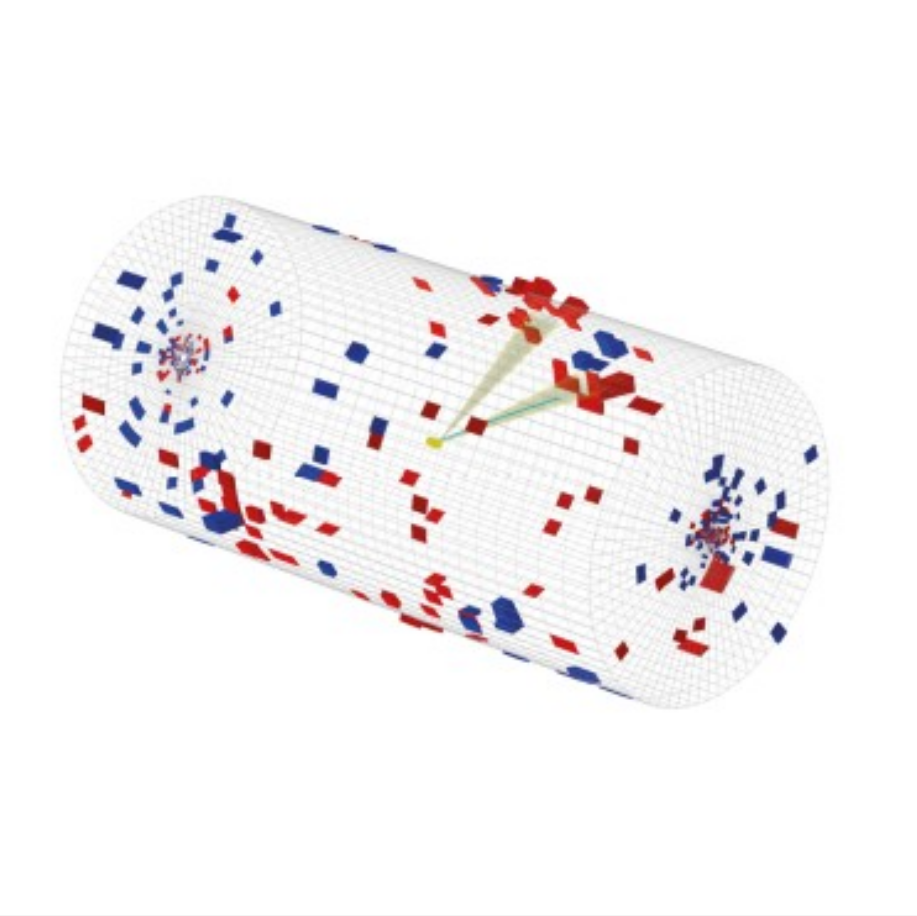
\includegraphics[width=\EmbedPictsWidth cm]{\PhDthesisdir/tex/slides/HTT_analysis/embedding_explained/remove_mumu.png}}};

\draw (\EmbedPictsWidth+\EmbedPictsMargin,-\EmbedPictsWidth/2-\EmbedPictsMargin) node [above left] {\EmbedPictsTxtSize Simulate $\Zboson\to\tau\tau$};
\draw (\EmbedPictsWidth+\EmbedPictsMargin,-\EmbedPictsWidth/2-\EmbedPictsMargin) node [below left] {\EmbedPictsTxtSize (\tau\ with same kinematics as \mu)};
\node[anchor=south west,inner sep=0] at (\EmbedPictsWidth+\EmbedPictsMargin,-\EmbedPictsWidth-\EmbedPictsMargin) {\frame{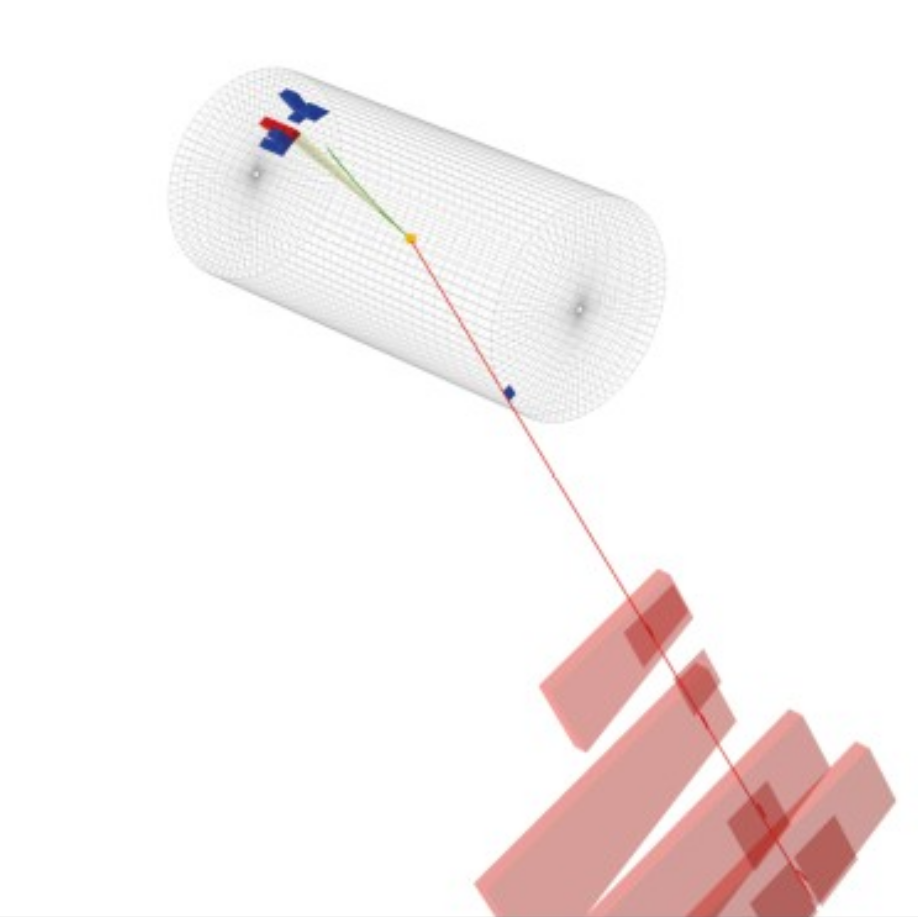
\includegraphics[width=\EmbedPictsWidth cm]{\PhDthesisdir/tex/slides/HTT_analysis/embedding_explained/Z_to_tautau_simulation.png}}};

%\draw [-latex, very thick] (2*\EmbedPictsWidth+6*\EmbedPictsMargin/5, \EmbedPictsWidth/4) -- (2*\EmbedPictsWidth+2*\EmbedPictsMargin-\EmbedPictsMargin/5,0);
%\draw [-latex, very thick] (2*\EmbedPictsWidth+6*\EmbedPictsMargin/5,-\EmbedPictsWidth/4-\EmbedPictsMargin) -- (2*\EmbedPictsWidth+2*\EmbedPictsMargin-\EmbedPictsMargin/5,-\EmbedPictsMargin);
%\draw (2*\EmbedPictsWidth+2*\EmbedPictsMargin+\EmbedPictsWidth/2,\EmbedPictsWidth/2-\EmbedPictsMargin/2) node [above] {\EmbedPictsTxtSize $\Zboson\to\tau\tau$ embedded event};
%\node[anchor=south west,inner sep=0] at (2*\EmbedPictsWidth+2*\EmbedPictsMargin,-\EmbedPictsWidth/2-\EmbedPictsMargin/2) {\frame{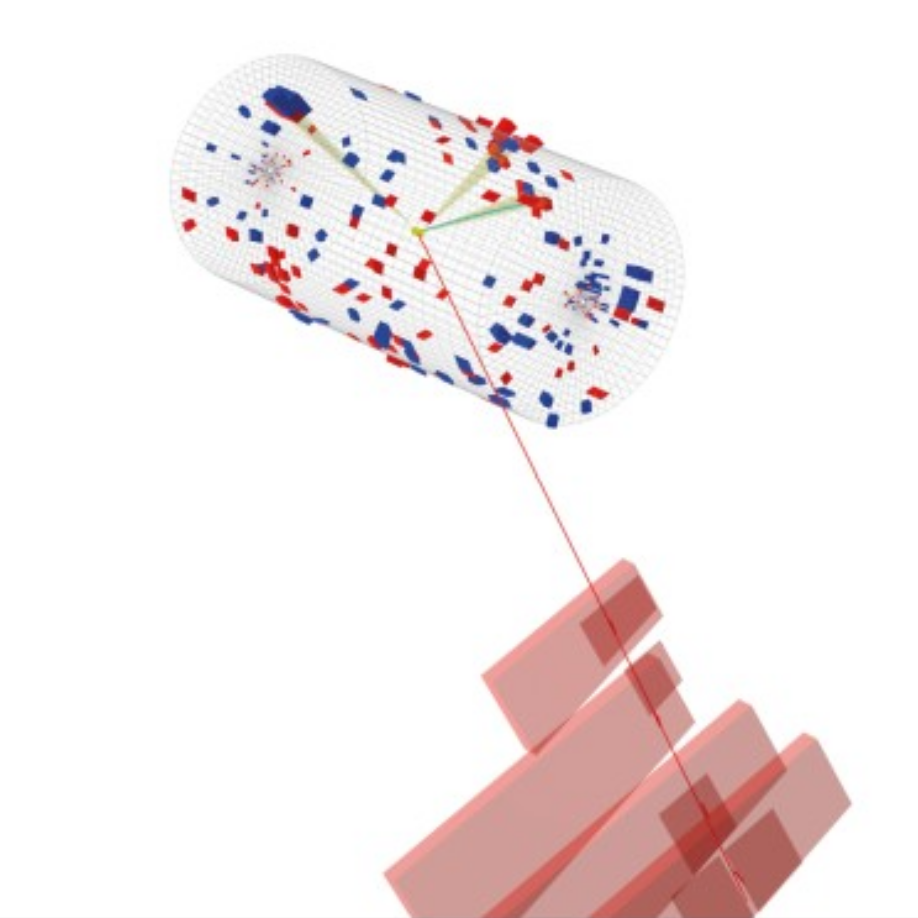
\includegraphics[width=\EmbedPictsWidth cm]{\PhDthesisdir/tex/slides/HTT_analysis/embedding_explained/embedded_event.png}}};

\clip (-1,-\EmbedPictsWidth-\EmbedPictsMargin-.25) rectangle (3*\EmbedPictsWidth+5*\EmbedPictsMargin/2+.25, \EmbedPictsWidth+.5);
\end{tikzpicture}
\end{center}
\end{frame}

\begin{frame}\addtocounter{framenumber}{-1}
\frametitle{Embedded events}
\begin{center}
\begin{tikzpicture}
\draw (\EmbedPictsWidth/2, \EmbedPictsWidth) node [above] {\EmbedPictsTxtSize $\Zboson\to\mu\mu$ data};
\node[anchor=south west,inner sep=0] at (0,0) {\frame{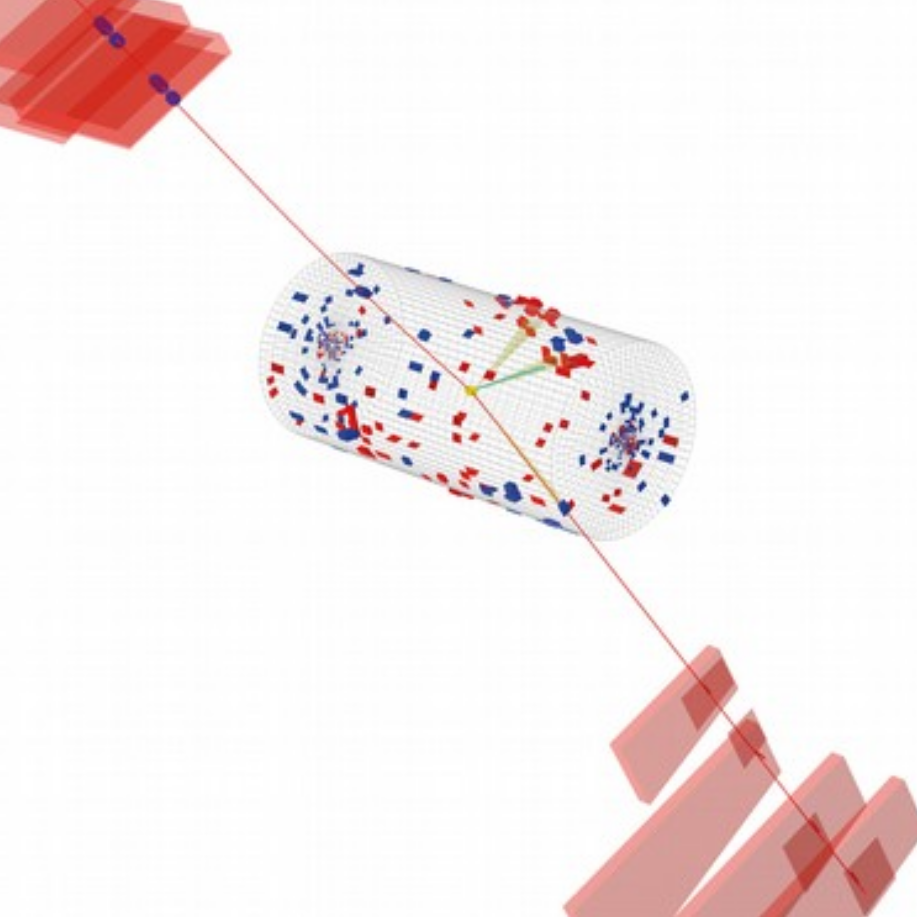
\includegraphics[width=\EmbedPictsWidth cm]{\PhDthesisdir/tex/slides/HTT_analysis/embedding_explained/Z_to_mumu_data.png}}};

\draw [-latex, very thick] (\EmbedPictsWidth+\EmbedPictsMargin/5, \EmbedPictsWidth/2) -- + (3*\EmbedPictsMargin/5,0);
\draw (\EmbedPictsWidth/2+\EmbedPictsWidth+\EmbedPictsMargin, \EmbedPictsWidth) node [above] {\EmbedPictsTxtSize Remove $\mu\mu$ system};
\node[anchor=south west,inner sep=0] at (\EmbedPictsWidth+\EmbedPictsMargin,0) {\frame{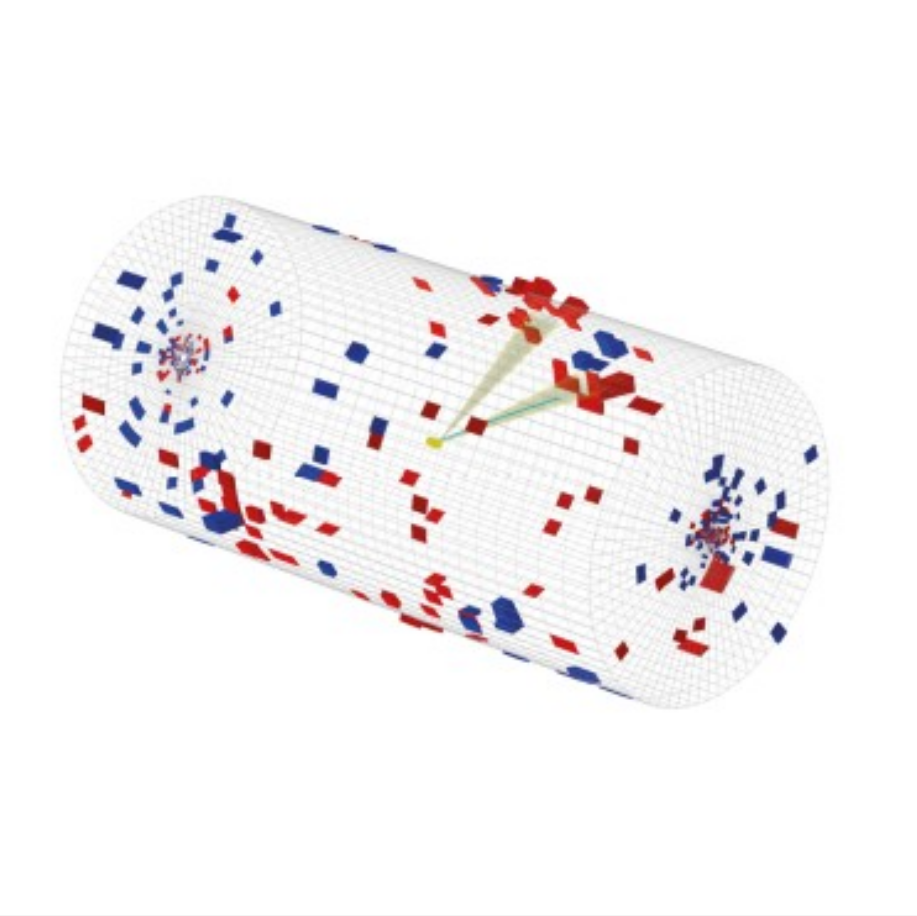
\includegraphics[width=\EmbedPictsWidth cm]{\PhDthesisdir/tex/slides/HTT_analysis/embedding_explained/remove_mumu.png}}};

\draw (\EmbedPictsWidth+\EmbedPictsMargin,-\EmbedPictsWidth/2-\EmbedPictsMargin) node [above left] {\EmbedPictsTxtSize Simulate $\Zboson\to\tau\tau$};
\draw (\EmbedPictsWidth+\EmbedPictsMargin,-\EmbedPictsWidth/2-\EmbedPictsMargin) node [below left] {\EmbedPictsTxtSize (\tau\ with same kinematics as \mu)};
\node[anchor=south west,inner sep=0] at (\EmbedPictsWidth+\EmbedPictsMargin,-\EmbedPictsWidth-\EmbedPictsMargin) {\frame{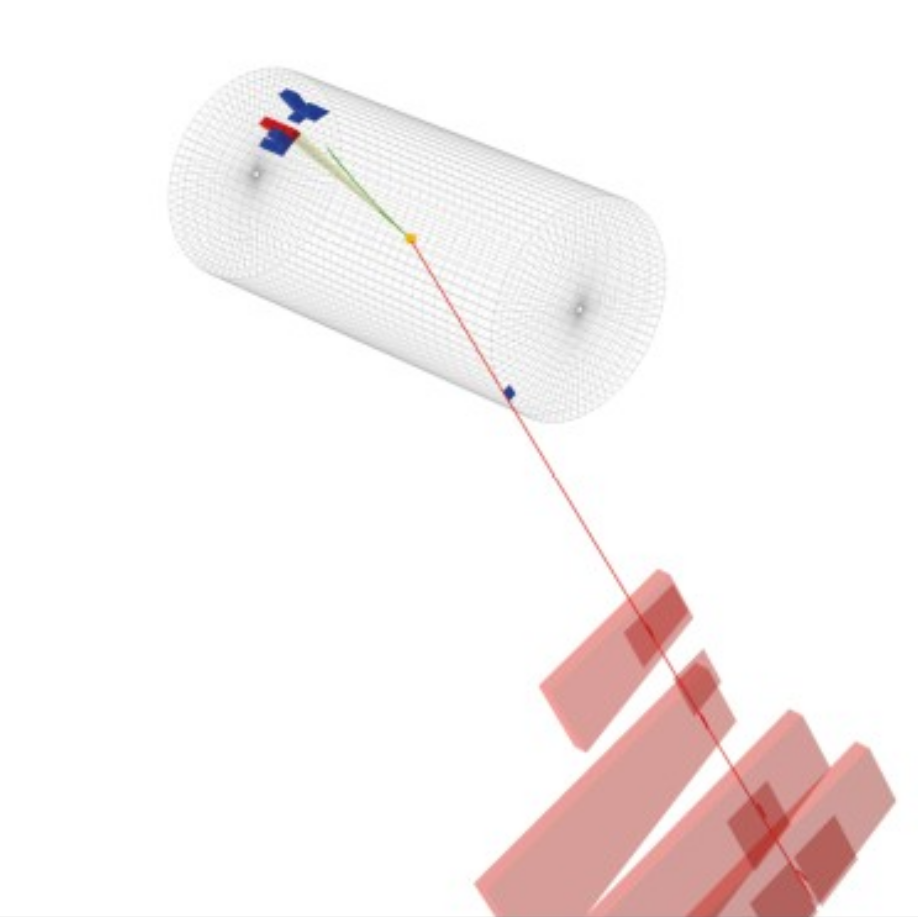
\includegraphics[width=\EmbedPictsWidth cm]{\PhDthesisdir/tex/slides/HTT_analysis/embedding_explained/Z_to_tautau_simulation.png}}};

\draw [-latex, very thick] (2*\EmbedPictsWidth+6*\EmbedPictsMargin/5, \EmbedPictsWidth/4) -- (2*\EmbedPictsWidth+2*\EmbedPictsMargin-\EmbedPictsMargin/5,0);
\draw [-latex, very thick] (2*\EmbedPictsWidth+6*\EmbedPictsMargin/5,-\EmbedPictsWidth/4-\EmbedPictsMargin) -- (2*\EmbedPictsWidth+2*\EmbedPictsMargin-\EmbedPictsMargin/5,-\EmbedPictsMargin);
\draw (2*\EmbedPictsWidth+2*\EmbedPictsMargin+\EmbedPictsWidth/2,\EmbedPictsWidth/2-\EmbedPictsMargin/2) node [above] {\EmbedPictsTxtSize $\Zboson\to\tau\tau$ embedded event};
\node[anchor=south west,inner sep=0] at (2*\EmbedPictsWidth+2*\EmbedPictsMargin,-\EmbedPictsWidth/2-\EmbedPictsMargin/2) {\frame{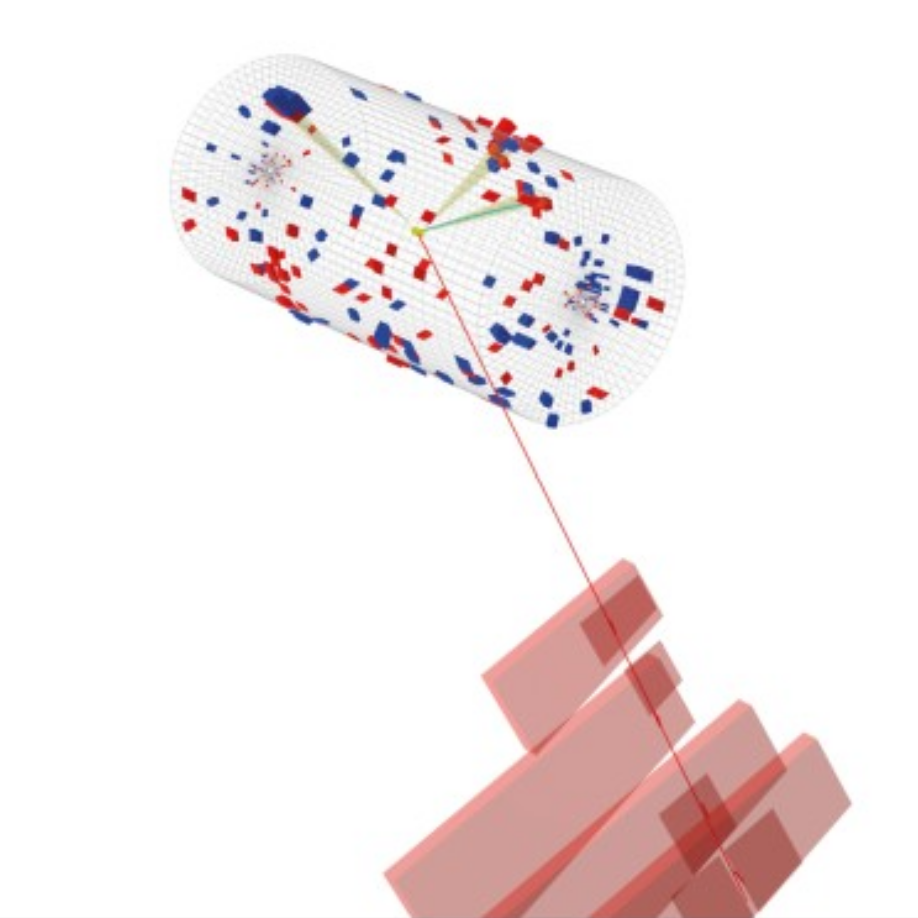
\includegraphics[width=\EmbedPictsWidth cm]{\PhDthesisdir/tex/slides/HTT_analysis/embedding_explained/embedded_event.png}}};

\clip (-1,-\EmbedPictsWidth-\EmbedPictsMargin-.25) rectangle (3*\EmbedPictsWidth+5*\EmbedPictsMargin/2+.25, \EmbedPictsWidth+.5);
\end{tikzpicture}
\end{center}
\end{frame}